\begin{center}
\indent
\textit{La loro teoria serve ad inquadrare la risoluzione dei sistemi di equazioni lineari. \\ Spazio vettoriale delle matrici, spazio vettoriale delle $n$-uple di numeri reali.}
\end{center}

\section{Spazi vettoriali su un campo $\field$}

Uno spazio vettoriale \`e una struttura algebrica $(V, +, \cdot)$ su un campo $\field$ le cui operazioni sono $+ : V \times V \to V$ e l'operazione ``esterna'' $\cdot : \field \times V \to V$. Il $\cdot$ \`e detto ``moltiplicazione esterna''. Gli elementi di $V$ si dicono \textit{vettori}.

Uno spazio vettoriale gode delle seguenti propriet\`a:
\begin{description}
    \item[1V] $(V, +)$ \`e un gruppo abeliano
    \item[2V] $\forall k \in \field$, $\forall v, w \in V$, $k \cdot (v + w) = k \cdot v + k \cdot w$. Questa propriet\`a \`e detta distributiva rispetto all'addizione in $V$ (ossia, rispetto all'addizione vettoriale).
    \item[3V] $\field$ \`e un campo, quindi $\forall k, h \in \field$ e $\forall v \in V$, $(k + h) \cdot v = k \cdot v + h \cdot v$. Questa propriet\`a \`e detta distributiva rispetto all'addizione in $\field$
    \item[4V] $\forall k, h \in \field$, $\forall v \in V$, $(h \cdot k ) \cdot v = h \cdot (k \cdot v) = k \cdot (h \cdot v)$. \`E una specie di propriet\`a associativa.
    \item[5V] $\forall v \in V$, $1 \cdot v = v$
\end{description}

Un elemento $k \in \field$ viene detto ``scalare''.

Gli spazi vettoriali danno una veste teorica alla risoluzione dei sistemi lineari.

\subsubsection{Esempi di spazi vettoriali}

Il nome degli spazi vettoriali viene dagli spazi vettoriali geometrici. $(V_O, +, \cdot)$ \`e lo spazio vettoriale su $\reals$ dei vettori dello spazio euclideo applicati in un punto $O$ (detto ``origine'').

La somma fra vettori geometrici si effettua con la ``regola del parallelogramma'' (figura \ref{fig:parallelogramma}). Le forze possono essere rappresentate dai vettori del piano.

\begin{figure}[ht]
\centering
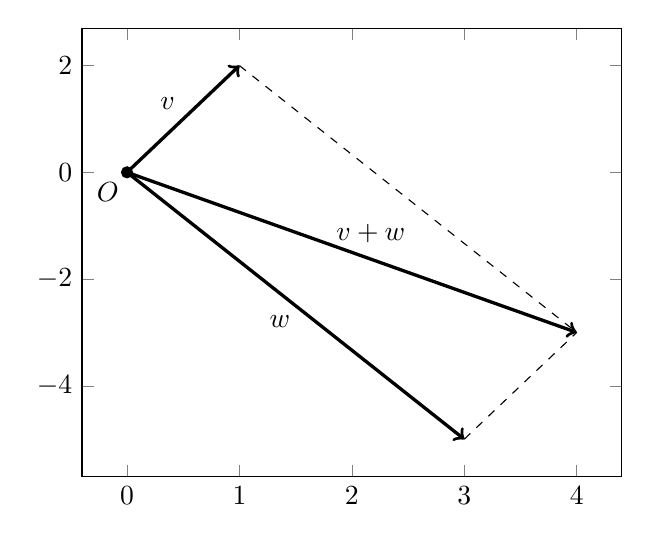
\begin{tikzpicture}
\begin{axis}[
    % graph options
]
\addplot [black, mark = *, nodes near coords=$O$,every node near coord/.style={anchor=45}] coordinates {( 0, 0)};
\addplot [black, nodes near coords=$v$,every node near coord/.style={anchor=315}] coordinates {( 0.5, 1)};
\addplot [black, nodes near coords=$w$,every node near coord/.style={anchor=45}] coordinates {( 1.5, -2.5)};
\addplot [black, nodes near coords=$v+w$,every node near coord/.style={anchor=225}] coordinates {( 2, -1.5)};
\addplot[very thick,->] coordinates {(0,0) (1,2)};
\addplot[very thick,->] coordinates {(0,0) (3,-5)};
\addplot[very thick,->] coordinates {(0,0) (4,-3)};
\addplot[dashed] coordinates {(1,2) (4,-3)};
\addplot[dashed] coordinates {(3,-5) (4,-3)};
\end{axis}
\end{tikzpicture}
\caption{\label{fig:parallelogramma}Metodo del parallelogramma}
\end{figure}

L'elemento neutro \`e il vettore nullo, i cui estremi coincidono in $O$, e si indica con $\underline{\underline{O}} = \overrightarrow{OO}$.  L'inverso di un vettore $v$ \`e chiamato $-v$, ha stessa direzione, stesso modulo e verso contrario.

Per creare lo spazio vettoriale abbiamo bisogno infine dell'operazione esterna: il prodotto scalare $ \cdot : \reals \times V \to V$ (figura \ref{fig:prodotto_scallare}).

\begin{figure}[ht]
\centering
\begin{tikzpicture}
\begin{axis}[
    % graph options
]
\addplot [black, mark = *, nodes near coords=$O$,every node near coord/.style={anchor=135}] coordinates {( 0, 0)};
\addplot [black, nodes near coords=$v$,every node near coord/.style={anchor=315}] coordinates {( 0.5, 1)};
\addplot [black, nodes near coords=$-v$,every node near coord/.style={anchor=315}] coordinates {( -0.5, -1)};
\addplot [black, nodes near coords=$2v$,every node near coord/.style={anchor=135}] coordinates {( 1.5, 3)};
% \addplot[only marks] coordinates {(0,0)}; % punto
\addplot[very thick,->] coordinates {(0,0) (1,2)};
\addplot[dashed,->] coordinates {(0,0) (-1,-2)};
\addplot[dashed,->] coordinates {(0,0) (2,4)};
\end{axis}
\end{tikzpicture}
\caption{\label{fig:prodotto_scallare}Prodotto scalare}
\end{figure}

Le $n$-uple degli elementi di un campo $\field$ sono uno spazio vettoriale, ossia $(\field^n, +, \cdot)$ \`e uno spazio vettoriale su $\field$. Se ad esempio il campo \`e $\reals$ e $n = 3$, prendiamo le terne di numeri reali $(a,b,c) \in \reals^3$. La somma di due terne \`e $(a,b,c) + (x,y,z) = (a + x, b + y, z + c)$. Moltiplicare una terna per un numero si chiama ``moltiplicare per uno scalare'', e $r \cdot (a,b,c) = (r \cdot a, r \cdot b, r \cdot c)$.

Anche i polinomi $(\field[x], +, \cdot)$ sono uno spazio vettoriale. Moltiplicare un polinomio per uno scalare (ossia per un elemento del campo) vuol dire moltiplicare tutti i coefficienti per lo scalare.

Abbiamo poi visto lo spazio vettoriale delle matrici. L'insieme delle matrici $(\matrices_{m \times n} (\field), +, \cdot)$ \`e uno spazio vettoriale. Date due matrici $A = (a_{i,j})$ e $B = (b_{i,j})$, la loro somma \`e $A + B = (a_{i,j} + b_{i,j})$, mentre la moltiplicazione per uno scalare $k$ \`e $k \cdot A = (k \cdot a_{i,j})$.

Dato un sottocampo di un campo $\subfield \subseteq \field$, ad esempio $\rationals \subseteq \reals \subseteq \complexes$, possiamo vedere $\field$ come spazio vettoriale su $\subfield$ (o anche su $\field$). $(\field, +, \cdot)$ ha l'operazione $\cdot : \subfield \times \field \to \field$, che dati $h \in \subfield$ e $ k \in \field \mapsto h \cdot k$.

\subsection{Sottospazi vettoriali}

Un sottoinsieme $W \subseteq V$, con $(V, +, \cdot)$ a indicare uno spazio vettoriale, si dice sottospazio di $V$ se $(W, +, \cdot)$ \`e ancora uno spazio vettoriale. Le operazioni devono essere $+ : W \times W \to W$, e $\cdot : \field \cdot W \to W$.

Condizione necessaria e sufficiente affinch\'e un insieme $W \subseteq V$ sia un sottospazio di $(V, +, \cdot)$ \`e che $W \neq \emptyset$, $\nullelement \in W$, e che:
\begin{align*}
\forall v, w \in W &\implies (v - w) \in W \\
\forall k \in \field , \, \forall w \in W &\implies k \cdot w \in W
\end{align*}

% Se $W$ \`e un sottospazio di $V$, (W, +) deve essere un sottogruppo di (V, +) \iff se prendo due vettori v, w \in W \implies (v - w) \in W. Poi bisogna vedere che \forall k \in \field e \forall w \in W \implies k \cdot w \in W. Quindi condizione necessaria e sufficiente affinch\'e un insieme W \subseteq V sia un sottospazio \`e che se W \neq \emptyset e \nullelement \in W, W deve verificare tutta la roba sopra.

Nello spazio dei vettori geometrici, quali sono i sottospazi? Deve contenere il vettore nullo. Quindi $W_0 = \{ \nullelement \}$ \`e un sottospazio banale. Se il sottospazio $W_1$ contiene un vettore $v \neq \nullelement$, deve contenere anche:
\begin{itemize}
    \item $0_{\field} \cdot v = \nullelement \in W_1$. Infatti $0_{\field} \cdot v = (0_{\field} + 0_{\field}) \cdot v = 0_{\field} \cdot v + 0_{\field} \cdot v \implies 0_{\field} \cdot v = \nullelement$
    \item $-1 \cdot v = -v$. Infatti $v + (-1) \cdot v = (1 - 1) \cdot v = 0_{\field} \cdot v = \nullelement$. Se moltiplico un vettore per $-1$ ottengo il suo opposto.
    \item deve contenere tutti i multipli $k \cdot v$, con $k \in \reals$.
\end{itemize}
Questo \`e un sottospazio, infatti verifica che $\forall v, w \in W_1 \implies v - w \in W_1$, e abbiamo visto che $\forall k \in \reals$, $k \cdot v \in W_1$.
\[
W_1 = \{ k \cdot v \in V : k \in \reals \}
\]
Un sottospazio quindi \`e il sottospazio dei vettori che hanno la stessa direzione di $v$, ossia \`e il sottospazio dei multipli di un vettore. Un sottospazio che contiene un vettore deve per forza contenere tutti i suoi multipli.

Vediamo cosa succede se il sottospazio contiene un vettore $w \neq k \cdot v$ con $k \in \reals$. Deve contenere anche tutti i multipli di $w$, per quanto appena visto. E deve quindi contenere le somme di tutti i vettori multipli di $v$ e di tutti i vettori multipli di $w$.
\[
W_2 = \{ a \cdot v + b \cdot w : a, b \in \reals \text{ e } v \neq k \cdot w \}
\]
$W_2$ sono tutti i vettori sul piano individuato dai vettori $v$ e $w$.

% disegnare vettore v, suo opposto, punto O, vettore w, direzione di v

Se aggiungiamo un terzo vettore diverso da $k \cdot v$ e $h \cdot w$ con $h, k \in \reals$, abbiamo che lo spazio vettoriale $W_3 \supseteq W_2$ \`e o $W_3 = W_2$ o $W_3 = V$. $W_2$ \`e detto ``massimale''.

Non esiste un sottospazio che lo contenga propriamente e che \`e diverso da tutto lo spazio.

Prendiamo l'insieme dei polinomi tali per cui il grado di $p(x) = n$.
\[
W_1 = \{ p(x) : \delta (p(x)) = n \}
\]
Non \`e un sottospazio: non contiene il polinomio nullo, e la differenza fra due polinomi non sempre ha grado $n$.
\[
W_2 = \{ p(x) : \delta (p(x)) \le n \}
\]
Questo \`e invece un sottospazio.
\[
W_3 = \{ p(x) : \delta (p(x)) \le 3 \text{ e } a_1 = a_2 = 0 \}
\]
Anche questo \`e un sottospazio. $\nullelement \in W_3$. La differenza fra due polinomi $a_0 + a_3 \cdot x^3 - b_0 - b_3 \cdot x^3 = a_0 - b_0 + (a_3 - b_3) \cdot x^3$ \`e ancora dentro $W_3$, quindi \`e un sottogruppo. Inoltre $k \cdot (a_0 + a_3 \cdot x^3)$ \`e $k \cdot a_0 + k \cdot a_3 \cdot x^3$, che \`e sempre in $W_3$.

Consideriamo ora $(\reals^4, +, \cdot)$, e il sottoinsieme:
\[
W = \{ (a_1, a_2, a_3, a_4) : a_1 + a_2 = 0 \}
\]
Prendiamo due elementi $(a_1, a_2, a_3, a_4)$ e $(b_1, b_2, b_3, b_4)$ e facciamo la differenza, ossia $(a_1 - b_1, a_2 - b_2, a_3 - b_3, a_4 - b_4)$. Vediamo che $a_1 - b_1 + a_2 - b_2$ \`e uguale a 0. Per verificare che \`e un sottospazio, dobbiamo verificare che una quaterna moltiplicata per $k$ \`e ancora dentro $W$.
\[
k \cdot (a_1, a_2, a_3, a_4) = (k \cdot a_1, k \cdot a_2, k \cdot a_3, k \cdot a_4)
\]
\`E verificato, infatti $k \cdot a_1 + k \cdot a_2 = k \cdot (a_1 + a_2) = k \cdot 0 = 0$.

\`E importante controllare sempre che il sottospazio sia vuoto, e che contenga il vettore nullo.
\[
W_1 = \{ (a_1, a_2, a_3, a_4) : a_1 = a_2^2 \}
\]
Questo non \`e un sottospazio, infatti non verifica che $k \cdot a_1 = k \cdot a_2^2$ , essendo $(k \cdot a_2)^2 = k^2 \cdot a_2^2 \neq k \cdot a_2^2$.

Consideriamo lo spazio vettoriale delle matrici quadrate $(\matrices_2 (\reals), +, \cdot)$.
\[
W = \left\{ 
\begin{smallpmatrix}
a & b  \\
c & d 
\end{smallpmatrix}
: a = 0 \right\}
\]
\`E un sottospazio, infatti $\nullelement = \begin{smallpmatrix}0&0\\ 0&0\end{smallpmatrix} $ \`e dentro $W$. Inoltre:
\[
k \cdot 
\begin{pmatrix}
0 & b \\
c & d
\end{pmatrix}
=
\begin{pmatrix}
0 & k \cdot b \\ 
k \cdot c & k \cdot d
\end{pmatrix}
\]
Consideriamo l'insieme:
\[
W_1 = \left\{
\begin{smallpmatrix}
a & b \\
c & d 
\end{smallpmatrix}
: a = d - 1 \right\} 
\]
Non \`e un sottospazio, poich\'e $\nullelement \notin W_1$.

\begin{prop}[Proposizione fondamentale per gli spazi vettoriali]
Siano $U, W$ sottospazi di $V \implies U \cap W$ \`e un sottospazio di $V$.
\end{prop}
Questo vale per tutte le strutture algebriche.

\begin{proof}
Vediamo che $\nullelement \in U \cap W$, essendo contenuto in entrambi.

Sia $v, w \in U \cap W \implies v - w \in U \cap W$, essendo $v - w \in U$ e $v - w \in W$.

Analogamente se $v \in U \cap W$ e $k \in \field \implies k \cdot v \in U \cap W$, essendo $U$ e $W$ sottospazi e quindi essendo ogni multiplo di $v$ in entrambi.
\end{proof}

\subsection{Reticolo dei sottospazi vettoriali}

Con i sottospazi vettoriali abbiamo un altro esempio di reticolo.

$\subgroupset(V)$ \`e l'insieme dei sottospazi dello spazio vettoriale $(V, +, \cdot)$. $(\subgroupset(V), \subseteq)$ \`e un reticolo, e $\subseteq$ indica la relazione di sottospazio. Siano $U, W \subseteq V$, l'$\inf$ di $U$ e $W$ \`e $U \cap W = U \infop W$. Verifica le propriet\`a dell'$\inf$, infatti se $T \subseteq U, W \implies T \subseteq U \cap W$.

Abbiamo gi\`a visto con i sottogruppi che l'unione di due sottogruppi in generale non \`e un sottogruppo. Anche qui, l'unione di due sottospazi non \`e, in generale, un sottospazio.

Abbiamo visto ad esempio che due sottospazi di $(V_O, +, \cdot)$ contenenti ciascuno i multipli di un solo vettore hanno un'unione che non \`e un sottospazio.

Il $\sup$ di $U$ e $W$, $U \supop W$, deve contenere l'unione di $U$ e $W$.
\[
U \subseteq U \cup W \subseteq U \supop W
\]
Inoltre sia $T$ un sottospazio di $V$ che contiene sia $U$ che $W$, $U, W \le T \implies U \supop W \le T$.

Quindi il $\sup$ \`e il pi\`u piccolo dei sottospazi che contiene l'unione. Quindi \`e l'intersezione di tutti i sottospazi che contengono sia $U$ che $W$.
\[
U \supop W = \bigcap_{U, W \subseteq T} T
\]
Vediamo come si caratterizza il $\sup$.

Abbiamo il reticolo dei sottospazi di uno spazio vettoriale.

Prendiamo un sottoinsieme $S$ dello spazio vettoriale $V$. Definiamo il sottospazio generato da da $S$. Lo indichiamo con $\pow{S}$. \`E definito come il pi\`u piccolo dei sottospazi contenenti $S$. $U \supop W$ \`e il sottospazio generato da $\pow{U \cup W}$.

Il sottospazio generato da $S$ \`e quindi:
\[
\pow{S} = \bigcap_{S \subseteq T} T
\]
Ossia l'intersezione di tutti i sottospazi contenenti $S$.

Prendendo $v \in V_O$, il sottospazio generato da $v$ \`e:
\[
\pow{v} = 
\begin{cases}
\nullelement \text{ se } v = \nullelement \\
\{ k \cdot v : k \in \field \} \text{ se } v \neq \nullelement
\end{cases}
\]

\subsection{Combinazioni lineari e indipendenza lineare}

Negli spazi vettoriali ci sono due concetti fondamentali da capire se si vuole capire qualcosa. Fissateli bene a mente, coglione.

\begin{description}
    \item[Combinazione lineare] Dati $n$ vettori $v_1, \dots v_n$ vettori di $V$, e $n$ scalari $k_1, \dots k_2 \in \field$, la combinazione lineare dei vettori $v_1 \dots v_n$ \`e un vettore:
    \[
    v = k_1 \cdot v_1 + \dots + k_n \cdot v_n
    \]
    Le combinazioni lineari di un solo vettore $v$ sono tutti i multipli del vettore $v$.
    \item[Indipendenza lineare] Si dice che un vettore $v$ dipende dai vettori $v_1, \dots v_t$ se $v \in \pow{\{v_1 \dots v_t\}}$, ossia se $v$ appartiene allo spazio generato da questi vettori, ossia $v$ si pu\`o scrivere come combinazione lineare dei vettori.
    \[
    v = a_1 \cdot v_1 + \dots + a_t \cdot v_t
    \]
    In caso contrario si dice che il vettore \`e indipendente linearmente, ossia non appartiene allo spazio generato.
\end{description}

\subsection{Esempi di combinazioni lineari}

Se prendiamo lo spazio vettoriale $(\reals^2, +, \cdot)$, un vettore qualunque $(a,b$) possiamo scriverlo come combinazione lineare dei vettori $(1,0)$ e $(0,1)$.
\[
(a,b) = a \cdot (1, 0) + b \cdot (0, 1)
\]
Un vettore di $\reals^3$ \`e formato da tutte le combinazioni lineari dei vettori $(1,0,0)$, $(0,1,0)$ e $(0,0,1)$.

In generale, un vettore di $\reals^n$ \`e formato dalla combinazione lineare di tutti i vettori $e_1 \dots e_n$ dove:
\[
e_i =
\begin{cases}
1 \text{ al posto } i \\
0 \text{ altrimenti}
\end{cases}
\]
Nello spazio dei polinomi $\reals[x]$, un polinomio $p(x)$ \`e combinazione lineare dei polinomi $\{ 1$, $x$, $x^2$, $\dots x^n$, $\dots \}$, ossia combinazione lineare dei polinomi $\{ x^i : i \in \naturals \}$.

Consideriamo le matrici quadrate di ordine 2, $\matrices_2 (\reals)$. Ogni matrice $\begin{smallpmatrix}a&b \\ c&d\end{smallpmatrix}$ \`e una combinazione lineare del tipo:
\[\
a \cdot
\begin{pmatrix}
1 & 0 \\
0 & 0 
\end{pmatrix}
+ b 
\begin{pmatrix}
0 & 1 \\
0 & 0 
\end{pmatrix}
+ c 
\begin{pmatrix}
0 & 0 \\
1 & 0 
\end{pmatrix}
+ d 
\begin{pmatrix}
0 & 0 \\
0 & 1
\end{pmatrix}
\]
Tutte le matrici nello spazio delle matrici quadrate di ordine 2 sono combinazione lineare delle matrici $\begin{smallpmatrix}1&0 \\ 0&0\end{smallpmatrix}$, $\begin{smallpmatrix}0&1 \\ 0&0\end{smallpmatrix}$, $\begin{smallpmatrix}0&0 \\ 1&0\end{smallpmatrix}$, $\begin{smallpmatrix}0&0 \\ 0&1\end{smallpmatrix}$.

In generale, tutte le matrici $\matrices_{m \times n} (\reals)$ sono combinazioni delle matrici $E_{h,k} (a_{i,j})$ dove:
\[
a_{i,j} = 
\begin{cases}
1 \text{ se } i = h \text{ e } j = k \\
0 \text{ altrimenti}
\end{cases}
\]
Nel caso di prima delle matrici quadrate di ordine 2, le matrici sono $E_{1,1}, E_{1,2}, E_{2,1}, E_{2,2}$.

Ritroviamo le combinazioni lineari negli spazi generati da sottoinsiemi di uno spazio vettoriale. $S$ \`e sottoinsieme dello spazio $(V, +, \cdot)$. $\Sigma (S)$ \`e insieme delle combinazioni lineari dei vettori di $S$. Quindi ogni $v \in \Sigma(S)$ \`e una combinazione lineare del tipo $v = a_1 s_1 + \dots + a_n s_n$ con $s_i \in S$.

\begin{prop}
$\pow{S}$, ossia lo spazio generato da $S$, \`e proprio $\Sigma(S)$.

$S$ \`e un sistema di generaotri di $\Sigma(S)$.
\end{prop}
\begin{proof}
Si dimostra per doppia inclusione. Banalmente $S \subseteq \Sigma(S)$, e $\Sigma(S)$ \`e un sottospazio di $V$. Infatti la differenza di due combinazioni lineari \`e in $\Sigma (S)$, cos\`i come il prodotto scalare di una combinazione lineare. Quindi $\pow{S} \subseteq \Sigma (S)$.

Dobbiamo far vedere che ogni combinazione lineare \`e contenuta in $\pow{S}$.
\[
v \in \Sigma(S) \implies v = a_1 \cdot s_1 + \dots a_n \cdot s_n \text{ con } s_i \in S
\]
$S$ \`e sottoinsieme di $T$, con $T$ sottospazio di $V$. $s_i \in T \forall i$, $a_i \cdot s_i \in T \forall i \implies v \in T$. $\Sigma(S) \subseteq T \forall T$ tale che $S \subseteq T$.
\end{proof}

Abbiamo quindi un'altra definizione del $\sup$ di due sottospazi.
\[
U \supop W = \pow{U \cup W} = \Sigma(U \cup W) = \bigcap_{U \cup W \subseteq T} T
\]
\begin{prop}
\[
(U \supop W) = U + W
\]
$U + W$ \`e l'insieme di tutti i vettori che posso scrivere come somma di $u + w$ con $u \in U$ e $w \in W$.
\[
U + W = \{ u + w : u \in U \text{ e } w \in W \}
\]
\end{prop}
\begin{proof}
Banalmente $U + W \subseteq \Sigma(U \cup W)$, ossia $U + W$ sono combinazioni lineari degli elementi di $U$ e $W$ in cui i coefficienti delle combinazioni lineari sono sempre 1.

Abbiamo anche che $U$ e $W \subseteq U + W$, che risulta essere un sottospazio.

Infatti prendendo gli elementi $(u + w)$ e $(u' + w')$, $(u + w) - (u' + w') = (u - u') + (w - w')$ \`e ancora in $U + W$. Poi $k \cdot (u + w) = k \cdot u + k \cdot w$ \`e dentro $U + W$.

Quindi se $U, W \subseteq U + W$, ed essendo $\Sigma(U \cup W)$ il pi\`u piccolo dei maggioranti di $U$ e $W$, deve essere che $U + W = \Sigma(U \cup W)$.
\end{proof}
\begin{prop}[Somma diretta fra spazi vettoriali]
$W$ e $U$ hanno somma diretta, che si indica con $U \oplus W$, se $ U \cap W = \{ \nullelement\}$. Le seguenti proposizioni sono equivalenti:
\begin{enumerate}
    \item\label{somma_diretta_1} $U$ e $W$ hanno somma diretta
    \item\label{somma_diretta_2} ogni vettore di $U + W$ si pu\`o esprimere in un unico modo come $u + w$, con $u \in U$ e $w \in W$
\end{enumerate}
\end{prop}
\begin{proof}
Il punto \ref{somma_diretta_1} implica il punto \ref{somma_diretta_2}.

Sia $v \in U + W$ tale che $v = u + w = \bar{u} + \bar{w}$, allora $u = \bar{u}$ e $w = \bar{w}$.

Infatti $(u + w) - (\bar{u} + \bar{w}) = \nullelement$. Da questo segue che possiamo scrivere $(u - \bar{u}) + (w - \bar{w}) = \nullelement$. Quindi $u - \bar{u} = - (w - \bar{w})$. Questo vettore si pu\`o scrivere come somma di due elementi di $U$ e come somma di due elementi di $W$, quindi \`e nell'intersezione. Quindi \`e il vettore nullo $\nullelement$, e quindi $u = \bar{u}$ e $w = \bar{w}$.

Ora vediamo che il punto \ref{somma_diretta_2} implica il punto \ref{somma_diretta_1}.

Dobbiamo dimostrare che l'intersezione contiene solo il vettore nullo. $U \cap W = \{ \nullelement \}$.

Consideriamo $v \in U \cap W$. Se $v \neq \nullelement$, dobbiamo scriverlo come somma di due vettori in $U$ e in $W$ in due modi diversi, cos\`i andiamo in contraddizione con l'ipotesi del punto \ref{somma_diretta_2}.

$v = \nullelement + v$ con $v \in W$, e $v = v + \nullelement$ con $v \in U$. Contraddizione.
\end{proof}

Se $W \oplus U = V$, i sottospazi $W$ e $U$ sono detti sottospazi supplementari.

Consideriamo lo spazio vettoriale delle matrici quadrate di ordine $n$, $(\matrices_n (\field), +, \cdot)$. $A$ \`e simmetrica se $A = A^t$, ossia se la matrice $A$ \`e uguale alla sua trasposta.
\[
A =
\begin{pmatrix}
1 & -1 & 2 \\
0 & 3 & 1 \\
3 & - & 10
\end{pmatrix}
\qquad
A^t =
\begin{pmatrix}
1 & 0 & 4 \\
-1 & 3 & -1 \\
2 & 1 & 0
\end{pmatrix}
\]
Se un elemento generico della matrice $A$ lo indico con $a_{i,j}$, un elemento generico della matrice trasposta si indica con $a_{j,i}$.

Una matrice $A$ si dice antisimmetrica se $A = -A^t$. Quindi l'elemento generico della matrice trasposta \`e $-a_{j,i}$, rispetto all'elemento generico della matrice antisimmetrica $A$ indicato con $a_{i,j}$.

Se prendiamo l'insieme di tutte le matrici quadrate simmetriche, $\matrices_{s}$, e l'insieme delle matrici quadrate antisimmetrice $\matrices_{a}$, questi sono due sottospazi dello spazio vettoriale delle matrici quadrate di ordine $n$, $ \matrices_n$.
\[
\matrices_s, \matrices_n \in \subgroupset \left( (\matrices_n (\field), +, \cdot) \right)
\]
Inoltre hanno somma diretta, e sono sottospazi supplementari.
\[
\matrices_{s} \oplus \matrices_{a} = \matrices_n (\field)
\]
Hanno intersezione contenente solo il vettore nullo: $\matrices_s \cap \matrices_a = \{ \nullelement \}$.

Come possiamo scrivere una matrice qualsiasi come somma di una matrice simmetrica e di una antisimmetrica? $A \in \matrices_n (\field)$ si scrive come:
\[
A = \frac{2 A}{2} = \frac{2 A - A^t + A^t}{2} = \frac{A + A^t}{2} - \frac{A - A^t}{2}
\]
La prima \`e simmetrica, la seconda \`e antisimmetrica.

Studieremo solo gli spazi vettoriali finitamente generati, cio\`e quelli per cui esiste un sottoinsieme finito $S$ tale che $\pow{S} = V$, ossia lo spazio generato da $S$ \`e uguale a tutto lo spazio vettoriale.

Ad esempio, lo spazio vettoriale di un campo $\field$ \`e generato da un solo elemento (l'unit\`a).

$\reals$ su $\reals$, $\complexes$ su $\complexes$, sono generati da un solo elemento. $\complexes$ su $\reals$ \`e generato da due elementi, un reale e un complesso. I due elementi sono $1$ e $i$.
\[
c = \{ x + y \cdot i : x, y \in \reals \} \in \complexes
\]
Le $n$-uple di elementi di un campo sono generate da $n$ vettori, ossia hanno un sistema di generatori di $n$ elementi. $\pow{\{e_1, \dots e_n\}} = \field^n$, dove:
\[
e_i = (x_1, \dots x_n) : x_j =
\begin{cases}
1 \text{ se } j = i \\
0 \text{ se } j \neq i
\end{cases}
\]
Lo spazio dei polinomi a valori in un campo non \`e finitamente generato.

Lo spazio delle matrici $m \times n$, $\matrices_{m \times n} (\field)$, \`e finitamente generato. Abbiamo gi\`a visto come si scrivono i suoi elementi.

\subsection{Indipendenza lineare}

\begin{defn}[Dipendenza dei sottospazi]
Un sottoinsieme di uno spazio vettoriale \`e dipendente se $\exists v \in S$ t.c. $v \in \pow{S \setminus \{v\}}$. Ossia lo spazio generato da $S \setminus \{v\}$ rimane uguale allo spazio generato da $S$.

Quindi un sottoinsieme $S$ \`e indipendente se $\forall v \in S, v \notin \pow{S \setminus \{v\}}$. Ossia $\pow{S} \neq \pow{S \setminus \{v\}}$.
\end{defn}

$S = \{ \nullelement \}$ \`e un sottoinsieme dipendente. $\pow{S \setminus \{ \nullelement \}} = \pow{\emptyset} = \pow{S} = \{ \nullelement \}$. In generale, ogni sottoinsieme contenente il vettore nullo \`e un sottoinsieme dipendente.

$S = \{ v \}$ con $v \neq \nullelement$ \`e sempre indipendente.

Se invece $S = \{ v_1, v_2 \}$, $S$ \`e dipendente se $v_1  = a \cdot v_2$, ossia se $v_1 \in \pow{v_2}$, altrimenti $S$ \`e indipendente.

La dipendenza dipende anche dal campo degli scalari.

Consideriamo lo spazio vettoriale di $\complexes$ su $\complexes$. $S = \{ 1, i \}$ \`e dipendente, perch\'e $i \cdot 1 = i$.

In $\complexes$ su $\reals$, invece, $S = \{1,i\}$ \`e indipendente (e genera pure tutto lo spazio).

Quindi lo stesso insieme di vettori, su spazi diversi, pu\`o avere una dipendeza o una indipendenza differente.

Consideriamo $(\field[x], +, \cdot)$ su $\field$, e l'insieme $S = \{ (1 - x), (1 + x^2), (1 + x - x^3) \}$.

Verifichiamo se $(1 - x) \in \pow{(1 + x^2), (1 + x - x^3)}$. Dobbiamo vedere se $(1 - x)$ si pu\`o scrivere come:
\[
a \cdot (1 + x^2) + b \cdot (1 + x + x^3) = ((a+b) + b \cdot x + a \cdot x^2 - b \cdot x^3) = (1 - x)
\]
Dovremmo risolvere il sistema in cui $a + b = 1$, $b = -1$, $a = 0$, $b = 0$. Questo sistema non ha soluzioni. Un giorno impareremo a risolvere questi sistemi.

Si vede subito che $(1 + x^2)$ non pu\`o essere dentro $\pow{(1 - x), (1 + x + x^3)}$, siccome il coefficiente di secondo grado di questi polinomi sar\`a sempre 0. Anche $(1 + x + x^3)$ non appartiene a $\pow{(1 - x), (1 + x^2)}$. Quindi l'insieme $S$ \`e indipendente.

Dobbiamo trovare un modo efficace ed efficiente per controllare se un insieme \`e dipendente o indipendente.
\[
S = \{ (1,1,1), (0,1,1), (5, -7, -7)\}
\implies
\pow{S \setminus \{(5, -7, -7)\}} = \{ (a, a+b, a+b) : a, b \in \reals \}
\]
Possiamo ritrovare $(5, -7, -7)$ in questo spazio? S\`i. Dobbiamo avere $a = 5$ e $a + b = -7$, quindi $b = -7 - 5 = -12$. Questo sottoinsieme \`e dipendente.

\subsection{Caratterizzazione degli insiemi indipendenti}

$S$ \`e indipendente $\iff \forall s_1, \dots, s_t \in S , \, a_1 \cdot s_1 + \dots + a_t \cdot s_t = \nullelement \implies a_1 = \dots = a_t = 0$, ossia l'unica combinazione lineare di vettori di $S$ uguale al vettore nullo \`e quella banale.

$S$ \`e dipendente $\iff \exists s_1, \dots s_t \in S$ tali che $a_1 \cdot s_1 + \dots + a_t \cdot s_t = \nullelement$ e $a_i \neq 0$ per qualche $i$, ossia esiste una combinazione lineare non banale di vettori di $S$ uguale al vettore nullo.

\begin{proof}
Vediamo che \`e condizione necessaria. Se $S$ \`e dipendente, $\exists v \in S$ tale che $v \in \pow{S \setminus \{v\}}$. Quindi $v = a_1 s_1 + \dots + a_t s_t$ dove $s_i \neq v$, essendo $s_i \in S \setminus \{v\}$. Quale combinazione lineare di vettori di $S$ \`e uguale al vettore nullo?
\[
a_1 s_1 + \dots + a_t s_t - v = \nullelement
\]
Vediamo che \`e condizione sufficiente, ossia se esiste una combinazione lineare non banale uguale al vettore nullo, allora $S$ \`e dipendente.
\[
\exists a_1 s_1 + \dots + a_t s_t = \nullelement
\]
Essendo non banale, possiamo supporre $a_1 \neq 0$. Prendiamo $v = a_1 s_1 = -(a_2 s_2 + \dots + a_t s_t)$. Quindi:
\[
v \in \pow{S \setminus \{v\}}
\]
Ossia, $S$ \`e dipendente.
\end{proof}
\[
S = \{ (1, 2, 2) , (1, -2, -1), (0, 4, 3) \}
\]
Per vedere se $S$ \`e dipendente, usiamo la caratterizzazione vista. Facciamo una combinazione lineare dei suoi elementi e vediamo se \`e uguale al vettore nullo.
\[
a \cdot (1, 2, 2) + b \cdot (1, -2, -1) + c \cdot (0, 4, 3) = \nullelement \implies
(a + b, 2a - 2b + 4c, 2a - b + 3c) = \nullelement
\]
Dobbiamo risolvere il seguente sistema lineare:
\[
\begin{cases}
a + b = 0 \\
2a - 2b + 4c = 0 \\
2a - b + 3c = 0
\end{cases}
\]
Risolvendo il sistema lineare abbiamo che le soluzioni sono $(a, -a, -a) \forall a \in \reals$. Quindi il sistema \`e dipendente.

\begin{fact}[Fatto fondamentale]
Sia $S$ un insieme indipendente, e $v$ un vettore non in $S$. Possiamo avere due casi:
\begin{itemize}
    \item $S \cup \{ v \}$ \`e dipendente $\iff v \in \pow{S}$
    \item $S \cup \{ v \}$ \`e indipendente $\iff v \notin \pow{S}$
\end{itemize}
Questa osservazione permette di costruire insieme indipendenti.
\end{fact}

Costruiamo un insieme $S$ indipendente in $\reals^3$. Partiamo da un insieme indipendente, contenente quindi un vettore diverso dal vettore nullo.
\[
v_1 = (1, -1, 2) \implies \pow{v_1} = \{ (a, -a, 2a) : a \in \reals \}
\]
Dobbiamo prendere $v_2 \notin \pow{v_1}$. Per farlo, assegnamo un valore ad $a$ e cambiamo una coordinata. Prendiamo, fissando $a = 2$, il vettore $(2, -2, 4)$. Sicuramente il vettore $(2, -2, 0)$ non \`e nello spazio generato da $v_1$.
\[
v_2 = (2, -2, 0)
\]
Quindi $S = \{ v_1, v_2 \}$ \`e ancora indipendente. Il suo spazio generato \`e:
\[
\pow{v_1, v_2} = \{ a \cdot v_1 + b \cdot v_2 : a, b \in \reals \} = 
\{ (a + 2b, -a -2b, 2a) : a, b \in \reals \}
\]
Possiamo trovare un vettore non in questo spazio, dando dei valori ad $a$ e $b$. Ad esempio $a = 1$ e $b = -1$, abbiamo il vettore $(-1, -3, 2)$. Il vettore $(-1, -3, 1)$ non \`e nell'insieme $S$. Quindi $S = \{(1, -1, 2), (2, -2, 0), (-1, -3, 1) \}$ \`e ancora indipendente.

Lo spazio generato da $S$ adesso \`e tutto $\reals^3$. Possiamo infatti vedere che ogni vettore generico $(a,b,c)$ si pu\`o scrivere come combinazione lineare dei tre vettori di $S$.
\[
\pow{S} = \{ (a + 2b - c, -a -2b -3c, 2a + c) : a, b, c \in \reals \}
\]
$S$ \`e un sistema di generatori minimale. Minimale vuol dire che non esiste un sistema di generatori pi\`u piccolo di $S$, ossia un $G \subseteq S$, tale che $\pow{G} = \reals^3$.

% SONO ARRIVATO QUI A CONTROLLARE

\subsection{Base di uno spazio vettoriale}

Il concetto di base di uno spazio vettoriale $(V, +, \cdot)$ su uno spazio $\field$ unisce i concetti di combinazione e indipendenza lineare.

\begin{defn}
Una base dello spazio vettoriale $(V, +, \cdot)$ \`e un sottoinsieme $B$ di $V$ tale che:
\begin{description}
    \item $B$ \`e indipendente
    \item $\pow{B} = V$, ossia $B$ \`e un sistema di generatori di $V$
\end{description}
\end{defn}

\begin{theorem}
Ogni spazio vettoriale $(V, +, \cdot)$ su un campo $\field$ ha (almeno) una base $B$, e tutte le basi hanno la stessa cardinalit\`a.
\end{theorem}
Se $\abs{B} = \infty$, si dice che $V$ ha dimensione infinita. Se invece $\abs{B} = n$, si dice che $V$ ha dimensione $n$. Si indica tipicamente con $\dim V = n$.

\begin{exmp}
$(\reals[x], +, \cdot)$ ha dimensione infinita. Infatti la base $B = \{ x^i : i \in \naturals \}$ ha cardinalit\`a infinita. Ogni polinomio $p(x)$ si scrive come combinazione lineare degli elementi di $B$, ossia:
\[
p(x) = a_0 + a_1 \cdot x + \dots + a_n \cdot x^n \text{ con } n = \delta(p(x))
\]
Gli elementi di $B$ sono indipendenti, infatti l'unica combinazione lineare degli elementi di $B$ che mi d\`a il vettore nullo $\nullelement$ \`e quella banale, ossia $\sum_{i = 0}^{\infty} a_i x^i = \nullelement \iff a_i = 0 \forall i$.

Consideriamo $\complexes$ su $\complexes$, o in generale lo spazio vettoriale di $\field$ su $\field$, abbiamo che $\dim_{\field} \field = 1$. Se invece consideriamo $\complexes$ su $\reals$, $\dim_{\reals} \complexes = 2$, infatti la sua base \`e $B = \{ 1, i \}$.

Considerando le matrici $m \times n$, $\left(\matrices_{m \times n}( \reals), +, \cdot \right)$, la sua dimensione \`e $\dim \matrices_{m \times n} (\reals) = m \times n$. La sua base \`e $B = \{ E_{i,j} : (i,j) \in [m] \times [n] \}$, dove la matrice generica \`e:
\[
E_{i,j} = (e_{h,k}) = 
\begin{cases}
1 \text{ se } (h,k) = (i,j) \\
0 \text{ altrimenti}
\end{cases}
\]
I polinomi di grado minore o uguale a $n$, ossia $(\reals_n [x], +, \cdot)$, hanno dimensione $\dim \reals_n[x] = (n+1)$.

Tutte le basi viste finora si chiamano \textbf{basi canoniche}.
\end{exmp}

\subsection{Caratterizzazione delle basi}

Le seguenti proposizioni sono equivalenti:
\begin{enumerate}
    \item\label{itm:basi_equiv_1} $B$ \`e una base di $(V, +, \cdot)$, ossia $\pow{B} = V$ e $B$ \`e indipendente
    \item\label{itm:basi_equiv_2} $B$ \`e un sistema di generazione minimale, ossia preso $S \subsetneqq B \implies \pow{S} \neq \pow{B} = V$
    \item\label{itm:basi_equiv_3} $B$ \`e un insieme indipendente massimale, ossia dato $S \supsetneqq B \implies S$ \`e dipendente, ossia non posso trovare un insieme pi\`u grande di $B$ che sia indipendente
\end{enumerate}

\begin{proof}
Dimostriamo che \ref{itm:basi_equiv_1} implica \ref{itm:basi_equiv_2}.

La tesi \`e che $B$ \`e minimale. Prendiamo un $S \subsetneqq B \implies \exists w \in B$ tale che $w \notin S$. Abbiamo quindi che:
\[
\pow{S} \subseteq \pow{B \setminus \{w\}} \subsetneqq \pow{B} = V
\]
Segue quindi che $\pow{S} \neq V$. $B$ \`e un sistema di generatori minimale (ossia ha il minimo numero di elementi).

Dimostriamo che \ref{itm:basi_equiv_2} implica \ref{itm:basi_equiv_3}.

Partendo dal fatto che $B$ \`e un sistema di generatori minimale, dobbiamo dimostrare che $B$ \`e un insieme indipendente massimale. $B$ \`e indipendente, perch\'e $\forall w \in B$, $\pow{B \setminus \{ w \}} \neq V$ essendo $B$ un sistema di generatori minimale.

Dobbiamo far vedere ora che dato un $S \supsetneqq B \implies S$ \`e dipendente. Infatti $\exists w \in S$ tale che $w \notin B$. Quindi $\pow{B} \subseteq \pow{S \setminus \{w\}} \subseteq \pow{S} = V$. $S$ \`e dipendente.

Dimostriamo che \ref{itm:basi_equiv_3} implica \ref{itm:basi_equiv_1}.

La tesi \`e che $\pow{B} = V$. Prendiamo un vettore qualunque $v \in V$ tale che $v \notin B$. $B \cup \{ v \}$ \`e dipendente, quindi esiste una combinazione lineare non banale di vettori di $B \cup \{ v \}$ che d\`a il vettore nullo. In particolare, questa combinazione lineare ha il coefficiente di $v$ diverso da 0. Quindi $v$ si pu\`o scrivere come combinazione lineare di vettori di $B$.
\[
a_1 v + a_2 v_2 + \dots + a_n v_n = \nullelement \implies
v = - \frac{a_2 v_2 + \dots + a_n v_n}{a_1}
\]
\end{proof}

\begin{prop}
Consideriamo lo spazio vettoriale $(V, +, \cdot)$ su $\field$. $B$ \`e una base se e solo se ogni vettore $v$ di $V$ si esprime in un solo modo come combinazione lineare di vettori di $B$.
\end{prop}
\begin{proof}
Vediamo che \`e condizione necessaria. L'ipotesi \`e che $B$ \`e una base. Supponiamo per assurdo che un vettore $v \in V$ si possa esprimere in due modi come combinazione lineare di elementi $e_i \in B$:
\[
v = a_1 \cdot e_1 + \dots + a_n \cdot e_n = b_1 \cdot e_1 + \dots + b_n \cdot e_n \implies
\nullelement = (a_1 - b_1) \cdot e_1 + \dots + (a_n - b_n) \cdot e_n
\]
Essendo $B$ indipendente, abbiamo che l'unica combinazione lineare che d\`a il vettore nullo \`e quella banale, quindi deve essere che $a_i = b_i \forall i$.

Dimostrare che \`e condizione sufficiente \`e molto pi\`u veloce. Sappiamo che ogni vettore di $V$ si esprime in un solo modo come combinazione lineare di elementi di $B$. Quindi banalmente $\pow{B} = V$. Inoltre, il vettore nullo si esprime in un solo modo:
\[
\nullelement = 0 \cdot e_1 + \dots + 0 \cdot e_n
\]
\end{proof}

\begin{oss}
Sia $(V, +, \cdot)$ uno spazio vettoriale sul campo $\field$ di dimensione $\dim_{\field} V = n$.
\begin{enumerate}
    \item $n$ vettori indipendenti sono una base
    \item $n$ generatori di $V$ costituiscono una base
    \item $(n+1)$ vettori costituiscono sempre un insieme dipendente
\end{enumerate}
\end{oss}

\begin{theorem}[Teorema del completamento]
Uno spazio vettoriale $(V, +, \cdot)$ sul campo $\field$ di dimensione $\dim_{\field} V = n$ e un insieme $S$ indipendente. Segue che $\abs{S} = t \le n$. Esistono $v_1 \dots v_h$ vettori (indipendenti) di $V$ tali che $S \cup \{ v_1 \dots v_k \}$ \`e una base, con $t + h = n$.
\end{theorem}
\begin{proof}
Se $\pow{S} = V \implies t = n$. Altrimenti, se $\pow{S} \neq V$, possiamo trovare un vettore $v_1 \notin \pow{S}$ tale che $S \cup \{ v_1 \}$ \`e indipendente. Si pu\`o ripetere il procedimento fino ad ottenere tutto $V$.

Prendiamo una base $B$ di $V$. Se $\pow{S} \neq V = \pow{B}$, allora $\exists v_1 \in B$ tale che $v_n \in \pow{S}$.
\end{proof}

\begin{theorem}[Teorema dell'estrazione]
Consideriamo un sottoinsieme $G \subseteq V$ tale che $\pow{G} = V$, ossia $G$ \`e un sistema di generatori di $V$. Possiamo trovare un sistema $S \subseteq G$ con $S = \{ v_1, \dots v_n \}$ tale che $G \setminus S$ \`e una base di $V$.
\end{theorem}
\begin{proof}
$\pow{G} = V$, ma $G$ non \`e una base. Quindi $\exists v_1 \in G$ tale che $\pow{G \setminus \{v_1\}} = V$, ossia $G \setminus \{ v_1 \}$ \`e sempre un sistema di generatori di $V$. Si pu\`o ripetere il procedimento fino ad ottenere una base, ossia finch\'e $G \setminus S$ \`e indipendente.

Se $\abs{G} = t$, dobbiamo togliere h vettori con $h = t - n$ e $\dim V = n$.

Alternativamente, prendiamo un vettore $v_1 \neq \nullelement$. $\{v_1\}$ \`e indipendente. Se $\pow{v_1} \neq V = \pow{G}$, allora $\exists v_2 \in G$ tale che $v_2 \notin \pow{v_1}$. Si ripete il ragionamento fino a trovare la base.
\end{proof}

\begin{exmp}
Nello spazio vettoriale $\reals^3$, prendiamo l'insieme $G = \{ (1, 0, 2), (-1, 1, 0), (1, 1, 4), (0, 1, 1) \}$. Il teorema dice che $\exists S \subseteq G$ tale che $G \setminus S$ \`e una base. La dimensione di $\reals^3$ \`e 3, quindi dobbiamo togliere un solo vettore.

$(1,0,2) \neq \nullelement$. Quindi L'insieme $\{ (1, 0, 2) \}$ \`e indipendente. $(-1, 1, 0)$ \`e indipendente da $(1, 0, 2)$, quindi anche l'insieme $\{ (1, 0, 2), (-1, 1, 0)\}$ \`e indipendente. I vettori nell'insieme generato da questi due vettori sono tutti nella forma $(a - b, b, 2a)$. Poniamo $a = 2$ e $b = 1$, e vediamo che il vettore $(1, 1, 4)$ \`e nello spazio generato da questi due. L'altro vettore $(0, 1, 1)$ non \`e generato dai due presi prima, quindi lo spazio $S = \{ (1, 0, 2), (-1, 1, 0), (0, 1, 1)\}$ \`e una base.

Consideriamo ora l'insieme $S = \{ (2, 1, 1), (2, -1, 1) \}$. Troviamo un vettore che aggiunto a $S$ faccia una base. Lo spazio generato da $S$ \`e:
\[
\pow{S} = \{ a (2, 1, 1) + b (2, -1, 1) : a, b \in \reals \} = \{ (2a + 2b, a - b, a + b) : a, b \in \reals \}
\]
Prima e terza coordinata sono ``dipendenti'', infatti $2a + 2b = 2 (a + b)$. Se fissiamo $a = 1$ e $b = 1$, ottenendo $(4, 0, 2)$, e cambiamo la seconda coordinata (che non \`e dipendente dalle altre due), otteniamo una $(4, 1, 2)$ che \`e nello spazio generato. L'equazione del nuovo vettore deve essere incompatibile.

La  coordinata da cambiare quindi non va scelta a caso, ma fra quelle dipendenti (se ce ne sono). 
\end{exmp}

Sia $B$ una base dello spazio vettoriale $(V, +, \cdot)$, abbiamo visto che ogni vettore $v$ di $V$ si esprime in un unico modo come combinazione lineare di vettori di $B$.
\[
v = a_1 \cdot v_1 + \dots + a_n \cdot v_n
\]
Ogni vettore si esprime come $n$-upla delle coordinate di $v$ rispetto a $B$, ossia $(a_1, \dots, a_n)$.

% SONO ARRIVATO QUI A SCRIVERE

















